%-----------------------------------
% Define document and include general packages
%-----------------------------------
% Tabellen- und Abbildungsverzeichnis stehen normalerweise nicht im
% Inhaltsverzeichnis. Gleiches gilt für das Abkürzungsverzeichnis (siehe unten).
% Manche Dozenten bemängeln das. Die Optionen 'listof=totoc,bibliography=totoc'
% geben das Tabellen- und Abbildungsverzeichnis im Inhaltsverzeichnis (toc=Table
% of Content) aus.
% Da es aber verschiedene Regelungen je nach Dozent geben kann, werden hier
% beide Varianten dargestellt.
\documentclass[12pt,oneside,titlepage,listof=totoc,bibliography=totoc]{scrartcl}
%\documentclass[12pt,oneside,titlepage]{scrartcl}

%-----------------------------------
% Dokumentensprache
%-----------------------------------
%\def\FOMEN{}% Auskommentieren um die Dokumentensprache auf englisch zu ändern
\newif\ifde
\newif\ifen

%-----------------------------------
% Meta information
%-----------------------------------
%-----------------------------------
% Meta Informationen zur Arbeit
%-----------------------------------

% Autor
\newcommand{\myAutor}{Sebastian Bunge}

% Adresse
\newcommand{\myAdresse}{Lindenstra\ss e 15c \\ \> \> \> 53227 Bonn}

% Titel der Arbeit
\newcommand{\myTitel}{Development of a Query Language for Full-Text Search in Relational Databases}

% Betreuer
\newcommand{\myBetreuer}{Prof. Dr. Peter Steininger}

% Lehrveranstaltung
\newcommand{\myLehrveranstaltung}{Modul}

% Matrikelnummer
\newcommand{\myMatrikelNr}{539441}

% Ort
\newcommand{\myOrt}{Bonn}

% Datum der Abgabe
\newcommand{\myAbgabeDatum}{\today}

% Semesterzahl
\newcommand{\mySemesterZahl}{7}

% Name der Hochschule
\newcommand{\myHochschulName}{FOM Hochschule für Oekonomie \& Management}

% Standort der Hochschule
\newcommand{\myHochschulStandort}{Bonn}

% Studiengang
\newcommand{\myStudiengang}{Wirtschaftsinformatik}

% Art der Arbeit
\newcommand{\myThesisArt}{Exposé}

% Zu erlangender akademische Grad
\newcommand{\myAkademischerGrad}{Bachelor of Science (B.Sc.)}

% Firma
\newcommand{\myFirma}{Deutsche Telekom IT GmbH}


\ifdefined\FOMEN
%Englisch
\entrue
\usepackage[english]{babel}
\else
%Deutsch
\detrue
\usepackage[ngerman]{babel}
\fi


\newcommand{\langde}[1]{%
   \ifde\selectlanguage{ngerman}#1\fi}
\newcommand{\langen}[1]{%
   \ifen\selectlanguage{english}#1\fi}
\usepackage[utf8]{luainputenc}
\langde{\usepackage[babel,german=quotes]{csquotes}}
\langen{\usepackage[babel,english=british]{csquotes}}
\usepackage[T1]{fontenc}
\usepackage{fancyhdr}
\usepackage{fancybox}
\usepackage[a4paper, left=4cm, right=2cm, top=4cm, bottom=2cm]{geometry}
\usepackage{graphicx}
\usepackage{colortbl}
\usepackage[capposition=top]{floatrow}
\usepackage{array}
\usepackage{float}      %Positionierung von Abb. und Tabellen mit [H] erzwingen
\usepackage{footnote}
% Darstellung der Beschriftung von Tabellen und Abbildungen (Leitfaden S. 44)
% singlelinecheck=false: macht die Caption linksbündig (statt zentriert)
% labelfont auf fett: (Tabelle x.y:, Abbildung: x.y)
% font auf fett: eigentliche Bezeichnung der Abbildung oder Tabelle
% Fettschrift laut Leitfaden 2018 S. 45
\usepackage[singlelinecheck=false, labelfont=bf, font=bf]{caption}
\usepackage{caption}
\usepackage{enumitem}
\usepackage{amssymb}
\usepackage{mathptmx}
%\usepackage{minted} %Kann für schöneres Syntax Highlighting genutzt werden. ACHTUNG: Python muss installiert sein.
\usepackage[scaled=0.9]{helvet} % Behebt, zusammen mit Package courier, pixelige Überschriften. Ist, zusammen mit mathptx, dem times-Package vorzuziehen. Details: https://latex-kurs.de/fragen/schriftarten/Times_New_Roman.html
\usepackage{courier}
\usepackage{amsmath}
\PassOptionsToPackage{table}{xcolor}\usepackage[most]{tcolorbox}
\tcbset{standard jigsaw, opacityback=0, colframe=black, sharp corners}
\usepackage{marvosym}			% Verwendung von Symbolen, z.B. perfektes Eurozeichen
\usepackage[nounderscore]{syntax}	% Write proper Backus-Naur Form, no underscore is needed to avoid problems with the cite function
\setlength{\grammarindent}{0pt}	% No indent in grammar to not having to use paragraphs and waste space

\renewcommand\familydefault{\sfdefault}
\usepackage{ragged2e}

% Mehrere Fussnoten nacheinander mit Komma separiert
\usepackage[hang,multiple]{footmisc}
\setlength{\footnotemargin}{1em}

% todo Aufgaben als Kommentare verfassen für verschiedene Editoren
\usepackage{todonotes}

% Verhindert, dass nur eine Zeile auf der nächsten Seite steht
\setlength{\marginparwidth}{2cm}
\usepackage[all]{nowidow}

%-----------------------------------
% Farbdefinitionen
%-----------------------------------
\definecolor{darkblack}{rgb}{0,0,0}
\definecolor{dunkelgrau}{rgb}{0.8,0.8,0.8}
\definecolor{hellgrau}{rgb}{0.0,0.7,0.99}
\definecolor{mauve}{rgb}{0.58,0,0.82}
\definecolor{dkgreen}{rgb}{0,0.6,0}

%-----------------------------------
% Pakete für Tabellen
%-----------------------------------
\usepackage{epstopdf}
\usepackage{nicefrac} % Brüche
\usepackage{multirow}
\usepackage{rotating} % vertikal schreiben
\usepackage{mdwlist}
\usepackage{tabularx}% für Breitenangabe

%-----------------------------------
% sauber formatierter Quelltext
%-----------------------------------
\usepackage{listings}
\usepackage{listings-rust}

\lstset{
	numbers=left,
	numberstyle=\tiny,
	numbersep=5pt,
	breaklines=true,
	showstringspaces=false,
	frame=l ,
	xleftmargin=5pt,
	xrightmargin=5pt,
	basicstyle=\ttfamily\small,
	stepnumber=1,
	keywordstyle=\color{blue},          % keyword style
  	commentstyle=\color{dkgreen},       % comment style
  	stringstyle=\color{mauve}         % string literal style
}

%-----------------------------------
%Literaturverzeichnis Einstellungen
%-----------------------------------

% Biblatex

\usepackage{url}
\urlstyle{same}

%%%% DIN 1505 Leitfaden
\usepackage[backend=biber, style=din, maxcitenames=2]{biblatex}%iso date format für YYYY-MM-DD

%% et al. anstatt u. a. bei mehr als drei Autoren.
\DefineBibliographyStrings{ngerman}{ 
	andothers = {{et\,al\adddot}},             
}
\DefineBibliographyStrings{english}{ 
	andothers = {{et\,al\adddot}},             
}

% Bib-Datei einbinden
% Replacement string for Zotero: \n\s+file = \{.*\},
\addbibresource{literatur/literatur.bib}

% Zeilenabstand im Literaturverzeichnis ist Einzeilig
% siehe Leitfaden S. 14
\AtBeginBibliography{\singlespacing}

%-----------------------------------
% Silbentrennung
%-----------------------------------
\usepackage{hyphsubst}
\HyphSubstIfExists{ngerman-x-latest}{%
\HyphSubstLet{ngerman}{ngerman-x-latest}}{}

%-----------------------------------
% Pfad fuer Abbildungen
%-----------------------------------
\graphicspath{{./}{./abbildungen/}}

%-----------------------------------
% Weitere Ebene einfügen
%-----------------------------------
\usepackage{titletoc}

\makeatletter

% Setze die Tiefe des Inhaltsverzeichnis auf 4 Ebenen
% Damit erscheinen \paragraph-Sektionen auch im Inhaltsverzeichnis
\setcounter{secnumdepth}{4}
\setcounter{tocdepth}{4}

% Fuege Abstand nach unten wie in einer normalen \section hinzu
% Andernfalls haette \paragraph keinen Zeilenumbruch
% Der Zeilenumbruch koennte mit einer leeren \mbox{} ersetzt werden
% Jedoch klebt dann der Text relativ nah an der Ueberschrift
\renewcommand{\paragraph}{%
  \@startsection{paragraph}{4}%
  {\z@}{3.25ex \@plus 1ex \@minus .2ex}{1.5ex plus 0.2ex}%
  {\normalfont\normalsize\bfseries\sffamily}%
}

\makeatother


%-----------------------------------
% Zeilenabstand 1,5-zeilig
%-----------------------------------
\usepackage{setspace}
\onehalfspacing

%-----------------------------------
% Absätze durch eine neue Zeile
%-----------------------------------
\setlength{\parindent}{0mm}
\setlength{\parskip}{0.8em plus 0.5em minus 0.3em}

\sloppy					%Abstände variieren
\pagestyle{headings}

%----------------------------------
% Präfix in das Abbildungs- und Tabellenverzeichnis aufnehmen, statt nur der Nummerierung (siehe Issue #206).
%----------------------------------
\KOMAoption{listof}{entryprefix} % Siehe KOMA-Script Doku v3.28 S.153
\BeforeStartingTOC[lof]{\renewcommand*\autodot{:}} % Für den Doppelpunkt hinter Präfix im Abbildungsverzeichnis
\BeforeStartingTOC[lot]{\renewcommand*\autodot{:}} % Für den Doppelpunkt hinter Präfix im Tabellenverzeichnis

%----------------------------------
% Rename list of to index of
%----------------------------------
\addto\captionsenglish{\renewcommand{\listfigurename}{Index of Figures}}
\addto\captionsenglish{\renewcommand{\listtablename}{Index of Tables}}

%-----------------------------------
% Abkürzungsverzeichnis
%-----------------------------------
\usepackage[printonlyused]{acronym}

%-----------------------------------
% Index of Symbols
%-----------------------------------
% Quelle: https://www.namsu.de/Extra/pakete/Listofsymbols.pdf
\usepackage[final]{listofsymbols}

%-----------------------------------
% Index of Formulae
%-----------------------------------
\DeclareCaptionType{mycapequ}[Formula][Index of Formulae]
\DeclareCaptionListFormat{mycapequlist}{Formula~#2:}
\captionsetup[mycapequ]{listformat=mycapequlist}

%-----------------------------------
% Index of Listings
%-----------------------------------
\DeclareCaptionType{mycapcode}[Code Listing][Index of Code Listings]
\DeclareCaptionListFormat{mycapcodelist}{Code Listing~#2:}
\captionsetup[mycapcode]{listformat=mycapcodelist}

%-----------------------------------
% PDF Meta Daten setzen
%-----------------------------------
\usepackage[hyperfootnotes=false]{hyperref} %hyperfootnotes=false deaktiviert die Verlinkung der Fußnote. Ansonsten inkompaibel zum Paket "footmisc"
% Behebt die falsche Darstellung der Lesezeichen in PDF-Dateien, welche eine Übersetzung besitzen
% siehe Issue 149
\makeatletter
\pdfstringdefDisableCommands{\let\selectlanguage\@gobble}
\makeatother

\hypersetup{
    pdfinfo={
        Title={\myTitel},
        Subject={\myStudiengang},
        Author={\myAutor},
        Build=1.1
    }
}

%-----------------------------------
% Umlaute in Code korrekt darstellen
% siehe auch: https://en.wikibooks.org/wiki/LaTeX/Source_Code_Listings
%-----------------------------------
\lstset{literate=
	{á}{{\'a}}1 {é}{{\'e}}1 {í}{{\'i}}1 {ó}{{\'o}}1 {ú}{{\'u}}1
	{Á}{{\'A}}1 {É}{{\'E}}1 {Í}{{\'I}}1 {Ó}{{\'O}}1 {Ú}{{\'U}}1
	{à}{{\`a}}1 {è}{{\`e}}1 {ì}{{\`i}}1 {ò}{{\`o}}1 {ù}{{\`u}}1
	{À}{{\`A}}1 {È}{{\'E}}1 {Ì}{{\`I}}1 {Ò}{{\`O}}1 {Ù}{{\`U}}1
	{ä}{{\"a}}1 {ë}{{\"e}}1 {ï}{{\"i}}1 {ö}{{\"o}}1 {ü}{{\"u}}1
	{Ä}{{\"A}}1 {Ë}{{\"E}}1 {Ï}{{\"I}}1 {Ö}{{\"O}}1 {Ü}{{\"U}}1
	{â}{{\^a}}1 {ê}{{\^e}}1 {î}{{\^i}}1 {ô}{{\^o}}1 {û}{{\^u}}1
	{Â}{{\^A}}1 {Ê}{{\^E}}1 {Î}{{\^I}}1 {Ô}{{\^O}}1 {Û}{{\^U}}1
	{œ}{{\oe}}1 {Œ}{{\OE}}1 {æ}{{\ae}}1 {Æ}{{\AE}}1 {ß}{{\ss}}1
	{ű}{{\H{u}}}1 {Ű}{{\H{U}}}1 {ő}{{\H{o}}}1 {Ő}{{\H{O}}}1
	{ç}{{\c c}}1 {Ç}{{\c C}}1 {ø}{{\o}}1 {å}{{\r a}}1 {Å}{{\r A}}1
	{€}{{\EUR}}1 {£}{{\pounds}}1 {„}{{\glqq{}}}1
}

%-----------------------------------
% Kopfbereich / Header definieren
%-----------------------------------
\pagestyle{fancy}
\fancyhf{}
% Seitenzahl oben, mittig, mit Strichen beidseits
% \fancyhead[C]{-\ \thepage\ -}

% Seitenzahl oben, mittig, entsprechend Leitfaden ohne Striche beidseits
\fancyhead[C]{\thepage}
%\fancyhead[L]{\leftmark}							% kein Footer vorhanden
% Waagerechte Linie unterhalb des Kopfbereiches anzeigen. Laut Leitfaden ist
% diese Linie nicht erforderlich. Ihre Breite kann daher auf 0pt gesetzt werden.
\renewcommand{\headrulewidth}{0.4pt}
%\renewcommand{\headrulewidth}{0pt}

%-----------------------------------
% Damit die hochgestellten Zahlen auch auf die Fußnote verlinkt sind (siehe Issue 169)
%-----------------------------------
\hypersetup{colorlinks=true, breaklinks=true, linkcolor=darkblack, citecolor=darkblack, menucolor=darkblack, urlcolor=darkblack, linktoc=all, bookmarksnumbered=false, pdfpagemode=UseOutlines, pdftoolbar=true}
\urlstyle{same}%gleiche Schriftart für den Link wie für den Text

%-----------------------------------
% Start the document here:
%-----------------------------------
\begin{document}

\pagenumbering{Roman}								% Seitennumerierung auf römisch umstellen
\newcolumntype{C}{>{\centering\arraybackslash}X}	% Neuer Tabellen-Spalten-Typ:
%Zentriert und umbrechbar

%-----------------------------------
% Textcommands
%-----------------------------------
%----------------------------------
%  TextCommands
%----------------------------------
%
%
%
%
%----------------------------------
%  common textCommands
%----------------------------------
% Information: OL bedeutet ohne Leerzeichen. Damit man dieses Command z. B. vor einem Komma oder vor einem anderen Zeichen verwenden kann. Dies ist ein Best-Practis von mir und hat sich sehr bewehrt.
% Allgemein hat es sich bewert alle Wörter die man häufig schreibt und wahrscheinlich falsch oder unterscheidlich schreibt, als Textcommand zu hinterlegen.
% 
%
%
\newcommand{\vglf}{\langde{Vgl.}\langen{C.f.}}
\newcommand{\pagef}{\langde{S. }\langen{p. }}
\newcommand{\os}{\mbox{o. S}}
\newcommand{\ojol}{\mbox{o. J.}}
\newcommand{\oj}{\ojol\ }
\newcommand{\og}{\mbox{o. g.}\ }
\newcommand{\ua}{\mbox{u. a.}\ }
\newcommand{\dah}{\mbox{d. h.}\ }
\newcommand{\zbol}{\mbox{z. B.}}
\newcommand{\zb}{\zbol\ }
\newcommand{\uamol}{unter anderem}
\newcommand{\uam}{\uamol\ }
\newcommand{\uanol}{unter anderen}%mit Leerzeichen
\newcommand{\uan}{\uanol\ }%mit Leerzeichen
\newcommand{\abbol}{Ab"-bil"-dung}
\newcommand{\abb}{\abbol\ }
\newcommand{\tabol}{Tabelle}
\newcommand{\tab}{\tabol\ }
\newcommand{\ggfol}{ggf.}
\newcommand{\ggf}{\ggfol\ }
\newcommand{\unodol}{und/oder}
\newcommand{\unod}{\unodol\ }


%-----------------------------------
% Titlepage
%-----------------------------------
\begin{titlepage}
	\newgeometry{left=2cm, right=2cm, top=2cm, bottom=2cm}
	\begin{center}
		
\includegraphics[width=2.3cm]{abbildungen/fomLogo} \\
		\vspace{.5cm}
		\begin{Large}\textbf{\myHochschulName}\end{Large}\\
		\vspace{.5cm}
		\begin{Large}\langde{Hochschulzentrum}\langen{university location} \myHochschulStandort\end{Large}\\
		\vspace{2cm}
		\begin{Large}\textbf{\myThesisArt}\end{Large}\\
		\vspace{.5cm}
		% \langde{Berufsbegleitender Studiengang}
		% \langen{part-time degree program}\\
		% \mySemesterZahl. Semester\\
		\langde{im Studiengang}\langen{in the study course} \myStudiengang
		\vspace{1.7cm}

		\langde{zur Erlangung des Grades eines}\langen{to obtain the degree of}\\
		\vspace{0.5cm}
		\begin{Large}{\myAkademischerGrad}\end{Large}\\
		% Oder für Hausarbeiten:
		%\textbf{im Rahmen der Lehrveranstaltung}\\
		%\textbf{\myLehrveranstaltung}\\
		\vspace{1.8cm}
		\langde{über das Thema}
		\langen{on the subject}\\
		\vspace{0.5cm}
		\large{\textbf{\myTitel}}\\
		\vspace{2cm}
		\langde{von}\langen{by}\\
		\vspace{0.5cm}
		\begin{Large}{\myAutor}\end{Large}\\
	\end{center}
	\normalsize
	\vfill
	\begin{tabular}{ l l }
		\langde{Betreuer} % für Hausarbeiten
		%\langde{Erstgutachter} % für Bachelor- / Master-Thesis
		\langen{Advisor}:              & \myBetreuer    \\
		\langde{Matrikelnummer}
		\langen{Matriculation Number}: & \myMatrikelNr  \\
		\langde{Abgabedatum}
		\langen{Submission}:           & \myAbgabeDatum
		\\
	\end{tabular}
\end{titlepage}


%-----------------------------------
% Inhaltsverzeichnis
%-----------------------------------
% Um das Tabellen- und Abbbildungsverzeichnis zu de/aktivieren ganz oben in Documentclass schauen
\setcounter{page}{2}
\addtocontents{toc}{\protect\enlargethispage{-20mm}}% Die Zeile sorgt dafür, dass das Inhaltsverzeichnisseite auf die zweite Seite gestreckt wird und somit schick aussieht. Das sollte eigentlich automatisch funktionieren. Wer rausfindet wie, kann das gern ändern.
\setcounter{tocdepth}{4}
\tableofcontents
\newpage

%-----------------------------------
% Abbildungsverzeichnis
%-----------------------------------
\listoffigures
\newpage

%-----------------------------------
% Tabellenverzeichnis
%-----------------------------------
\listoftables
\newpage

%-----------------------------------
% Abkürzungsverzeichnis
%-----------------------------------
\addcontentsline{toc}{section}{\abbreHeadingName}

\section*{\langde{Abkürzungsverzeichnis}\langen{List of Abbreviations}}

\begin{acronym}[EBNF]\itemsep0pt %der Parameter in Klammern sollte die längste Abkürzung sein. Damit wird der Abstand zwischen Abkürzung und Übersetzung festgelegt
  \acro{APT}{Automatically Programmed Tools}
  \acro{DDL}{Data Definition Language}
  \acro{DSL}{Domain-Specific Language}
  \acro{EBNF}{Extended Backus-Naur Form}
  \acro{GPL}{General-Purpose Language}
  \acro{HTML}{Hypertext Markup Language}
  \acro{MS}{Microsoft}
  \acro{PDF}{Portable Document Format}
  \acro{SQL}{Structured Query Language}
  \acro{XML}{Extensible Markup Language}
\end{acronym}
\newpage

%-----------------------------------
% Index of Symbols
%-----------------------------------
\addcontentsline{toc}{section}{\symheadingname}
\opensymdef
\newsym[precision]{symp}{p}
\newsym[recall]{symr}{r}
\newsym[number of relevant retrieved documents]{symn}{n}
\newsym[total number of retrieved documents]{symd}{d}
\newsym[total number of relevant documents]{symv}{v}
\newsym[weighted harmonic mean]{symFb}{F_{\beta}}
\newsym[nonnegative weight]{symbeta}{\beta}
\closesymdef
\listofsymbols
\newpage

%-----------------------------------
% Index of Formulae
%-----------------------------------
\listofmycapequs
\newpage

%-----------------------------------
% Index of Formulae
%-----------------------------------
\listofmycapcodes
\newpage

%-----------------------------------
% Seitennummerierung auf arabisch und ab 1 beginnend umstellen
%-----------------------------------
\pagenumbering{arabic}
\setcounter{page}{1}

%-----------------------------------
% Kapitel / Inhalte
%-----------------------------------
% Die Kapitel werden über folgende Datei eingebunden
% Hinzugefügt aufgrund von Issue 167
%-----------------------------------
% Kapitel / Inhalte
%-----------------------------------
\section{Abstract}
Abstract
\newpage
\section{Full-Text Search}
Commercial database management has long focused on structured data and the industry requirements have matched those of structured storage applications quite well.
The problem is that only a small part of the data stored is completely structured, while most of it is completely unstructured or only semi-structured, in the form of documents, emails, web pages, etc. \parencite[cf.][p. 7]{hamilton_microsoft_2001}\\
\subsection{MS SQL Server Search Architecture}
\ac{SQL} Server uses the same access method and infrastructure for full-text search as other \ac{MS} products and the Index Service for file systems. This decision enables standardized semantics for full-text search of data in relational databases, web-hosted data, and data stored in the file system and mail systems. On \ac{SQL} servers, not only simple strings can be indexed, but also data structures, such as \ac{HTML} and \ac{XML}, and even complex documents, such as \ac{PDF}, Word, PowerPoint, Excel and other custom document formats. \parencite[cf.][p. 7]{hamilton_microsoft_2001}\\
The architecture can be divided into five modules, which interact with each other to perform a full-text search. (See Figure \ref{fig:sql_search_architecture})\\
The \textbf{content reader} scans indexed data stored in \ac{SQL} Server tables to assemble data and its associated metadata packets. These packets are then injected into the main search engine, which triggers the search engine filter daemon to consume the data.\\
Depending on the content, the \textbf{filter daemon} calls different filters, which parse the content and output so-called chunks of the processed text. A chunk is a related section with relevant information about this section like the language-id of the text. These chunks are output separately for any properties, which can be elements like the title, an author or other content-specific elements.
\begin{figure}[H]
    \caption{Architecture of MS SQL Server Full-Text Search}
    \label{fig:sql_search_architecture}
    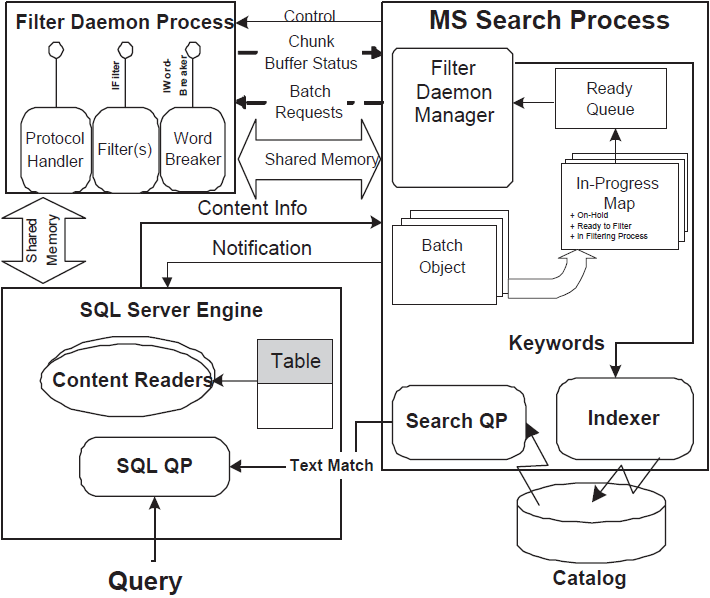
\includegraphics[width=0.9\textwidth]{sql_search_architecture.png}
    \\
    \cite[Source:][p. 8]{hamilton_microsoft_2001}
\end{figure}
\textbf{Word breakers} split the chunks into keywords and additionally provide alternative keywords and the corresponding position in the text. Word breakers can recognize human languages and on \ac{SQL} Server several word breakers for different languages are installed by default. The generated keywords and metadata are passed on to the \ac{MS} Search process, which processes the data with an indexer.\\
The \textbf{indexer} generates an inverted keyword list with a batch containing all keywords of one or more items. These indexes are compressed to use memory efficiently, this may lead to high costs for updates of these indexes. Therefore a stack of indexes is maintained. New documents first create their small indexes, which are regularly merged into a larger index, which in turn is merged into the base index. This stack can be deeper than three, but the concept remains and allows a strongly compressed index without driving the update costs too high. If a keyword is searched, all indexes are accessed, so the depth should still be kept reasonable.\\
A \textbf{query processor} manages the insertion and merge operations and collects statistics on distribution and frequency for ranking purposes and query execution. \parencite[cf.][pp. 8-9]{hamilton_microsoft_2001}
\subsection{MS SQL Server Full-Text Query Features}
Full-text indexes can be created on \ac{SQL} Servers with the \ac{DDL} statement \lstinline[language=SQL]$CREATE INDEX$ and can make use of other \ac{SQL} Server utilities; these include backup and restore and attachment of databases. There are three options to create and manage indexes on \ac{SQL} Servers. \textbf{Full Crawl} always rebuilds the whole full-text index by scanning the entire table. \textbf{Incremental Crawl} logs the timestamp of the last re-index and retains changes by storing them in a column. \textbf{Change Tracking} enables a near real-time validity between the full-text index and the table by tracking changes to the indexed data using the \ac{SQL} Server Query Processor. \parencite[cf.][p. 9]{hamilton_microsoft_2001}\\
Full-text search is represented in \ac{SQL} with three possible constructs: \parencite[cf.][p. 9]{hamilton_microsoft_2001}
\begin{enumerate}
    \item Contains Predicate: A contains predicate is true if one of the specified columns contains terms that satisfy the specified search condition. E.g. \lstinline[language=SQL]$Contains(author, ('Ag* or "Marc Miller"'))$ will match entries where the column author contains words like 'Ag', 'Agatha', or 'Marc Miller'.
    \item Freetext Predicate: Freetext predicates are true if one of the specified columns contains terms that stem from the terms in the specified search condition. E.g. \lstinline[language=SQL]$Freetext(content, 'fishing')$ will match entries where content contains words like 'fishing', 'fish', or 'fisher'.
    \item ContainsTable and FreetextTable: ContainsTable and FreetextTable are functions that match entries similar to their corresponding function, but additionally return multiple matches including a ranking for each entry and the entire corpus.
\end{enumerate}
The search conditions of these constructs can be of various types to find the intended results: \parencite[cf.][p. 9]{hamilton_microsoft_2001}
\begin{enumerate}
    \item Keyword, phrase, prefix: E.g. 'fishing', 'Marc Miller', 'Ag*'
    \item Inflections and Thesaurus: E.g. \lstinline[language=SQL]$Contains(*, 'FORMSOF(INFLECTIONAL, fishing) AND FORMSOF(THESAURUS, boat)')$ will find all entries containing words that stem from 'fishing' and all words sharing the meaning with 'boat' (Thesaurus support).
    \item Weighted terms: Keywords and phrases can be assigned a relative weight to impact the rank of entries. E.g. \lstinline[language=SQL]$ContainsTable(*, 'ISABOUT(generator weight (.7), full-text weight (.3))')$ will rank entries higher in the result corpus which mention 'generator' over 'full-text'.
    \item Proximity: E.g. \lstinline[language=SQL]$Contains(*, 'corn NEAR salad')$ contains the proximity term 'NEAR' to match entries where 'corn' appears close to 'salad'.
    \item Composition: E.g. \lstinline[language=SQL]$Contains(*, 'full-text AND NOT database')$ uses two search query components that are composed using a term like 'AND', 'OR', or 'AND NOT'.
\end{enumerate}

\subsection{Domain-Specific Languages}
Commonly known programming languages, such as C or Java, are also called a \ac{GPL}. \ac{GPL}s are designed to handle any problem with relatively equal levels of efficiency and expressiveness. However, many applications do not require a multifunctional \ac{GPL} and can describe a problem more naturally using a \ac{DSL}. \ac{DSL}s are languages that have been developed specifically for a particular application or domain, to be able to develop faster and more effectively. \parencite[cf.][p. 1]{hudak_domain-specific_1997}
By tailoring notations and constructs to the domain in question, \ac{DSL}s offer significant gains in expressiveness and usability compared to \ac{GPL}s for the domain in question, with corresponding productivity gains and lower maintenance costs. \parencite[cf.][p. 317]{mernik_when_2005}
\ac{DSL}s are by no means a product of modern software development but have existed since the beginning of programming. One of the first \ac{DSL}s ever designed was \ac{APT}, which was used for the development of numerically controlled machine tools in 1957. \parencite[cf.][pp. 283-284]{wexelblat_origins_1978}\\
\ac{DSL}s can be found everywhere in the world of IT, for example, this thesis was written with the help of \LaTeX{} to design layout and formatting. Table \ref{tbl:popular_dsl} lists some well-known \ac{DSL}s and their application/domain to give examples of what is classified as a \ac{DSL}.
\begin{table}[H]
    \caption{Popular DSLs}
    \label{tbl:popular_dsl}
    \begin{tabularx}{\textwidth}[ht]{|l|X|l|}
        \hline
        \textbf{DSL} & \textbf{Applicaiton} \\
        \hline
        Lex and Yacc & program lexing and parsing \\
        PERL & text/file manipulation/scripting \\
        VDL & hardware description \\
        \TeX, \LaTeX, troff & document layout \\
        HTML, SGML & document markup \\
        SQL, LDL, QUEL & databases \\
        pic, postscript & 2D graphics \\
        Open GL & high-level 3D graphics \\
        Tcl, Tk & GUI scripting \\
        Mathematica, Maple & symbolic computation \\
        AutoLisp/AutoCAD & computer aided design \\
        Csh & OS scripting (Unix) \\
        IDL & component technology (COM/CORBA) \\
        Emacs Lisp & text editing \\ 
        Prolog & logic \\
        Visual Basic & scripting and more \\
        Excel Macro Language & spreadsheets and many things never intended \\
        \hline
    \end{tabularx} \\
    \cite[Source:][p. 3]{hudak_domain-specific_1997}
\end{table}
Programs written in a \ac{DSL} are considered to be more concise, quicker to write, easier to maintain and easier to reason about and most importantly they can be written by non-programmers. In particular, experts in the domain for which the \ac{DSL} was developed can use \ac{DSL}s to program applications without having to acquire programming skills. An expert of a domain already knows the semantics of the domain, all that is needed to start development is the corresponding notation that expresses these semantics. \parencite[cf.][pp. 2-4]{hudak_domain-specific_1997}

\subsection{Building a language}
For a compiler or an interpreter to be able to interpret a \ac{DSL}, the language must be accurately and precisely defined. Accurately means that the language must be defined consistently down to the smallest detail. Precisely means in this case that all aspects of the language must be laid out. If parts of the language are inconsistent or too vague, authors of compilers are forced to interpret these aspects themselves. This inevitably leads to different authors having different approaches to the same problem. If a \ac{DSL} is to be created that meets the criteria described above, two components are needed. The first component is a set of rules, also called syntax. The second component is a formal definition of the meaning, also called semantics. \parencite[cf.][p. 2]{farrell_compiler_1995}
\subsubsection{Syntax}
The first step when defining syntax is defining an alphabet. This alphabet consists of tokens, which do not necessarily have to be letters. Several tokens, formulated according to a set of rules, make up a sentence or string. The alphabet of the English language is, in the context of syntax, not a list of the permissible characters, which is predominantly called the alphabet or 'ABC', but the permissible tokens.
E.g. in the sentence 'the donkey screams' the tokens 'the', 'donkey' and 'screams' are part of the alphabet of the English language. The token 'gHArFk' consists of permissible characters but is not part of the valid alphabet. However, the use of permissible tokens alone does not make a sentence correct. The sentence 'on sleep blue' consists of tokens that are part of the English alphabet, but it is still not a valid sentence. The correct application of the rule set is still missing, in this example a missing object. Only the correct use of the alphabet AND the set of rules make a sentence syntactically correct. \parencite[cf.][p. 2]{farrell_compiler_1995}\\
If the alphabet and the set of rules are notated in a normal form, they can be called grammar. Relevant to this thesis is the \ac{EBNF}, which will be described in section \ref{sec:EBNF}.
\subsubsection{Extended Backus-Naur Form}\label{sec:EBNF}
\ac{EBNF}, as the name suggests, is based on the Backus-Naur Form, which was proposed by a group of thirteen international representatives in 1960, to serve as a basic reference and guide for building compilers. Backus-Naur Form is a notation for describing computational processes and rules as arithmetic expressions, variables, and functions. \parencite[cf.][p. 300]{backus_report_1960}\\
The syntax can be described as a set of metalinguistic formulae best described with an example. The grammar describing a number can be written in Backus-Naur Form as:
\begin{grammar}
    <number> ::= <positive>|-<positive>|0 \\
    <positive> ::= <digit not zero><optional> \\
    <optional> ::= <digit><optional>| \\
    <digit> ::= <digit not zero>|0 \\
    <digit not zero> ::= 1|2|3|4|5|6|7|8|9
\end{grammar}
Characters contained in angel brackets '<>' represent a metalinguistic variable. The character '::=' describes a definition of this variable. The character '|' represents the metalinguistic connective 'or'. Other characters in this example have no special meaning but only represent themselves. So the first line of the grammar means that the variable <number> can be defined or replaced as <positive> or -<positive> or as 0. Since the variable <positive> is mentioned in the definition, there must be a definition for this variable in the grammar, otherwise, the grammar would be incomplete. In the third line, we see a metalinguistic connective without content on its right side. This means that the variable <optional> can also be empty and thus without value. Furthermore, in this line, a variable calls itself recursively, which is allowed. \parencite[cf.][pp. 301-303]{backus_report_1960}\\
So following this grammar, numbers such as 42 or -3141592 are valid.\\
In 1977 Wirth proposed a new variant of the Backus-Naur Form to further improve language definition notation. The main goals of this new notation were to \parencite[cf.][p. 822]{wirth_what_1977}
\begin{itemize}[noitemsep]
    \item distinguish clearly between metaterminal and nonterminal symbols
    \item not exclude metaterminals as possible symbols of the language
    \item enable iteration without using recursion
\end{itemize}
This proposal was the basis for the ISO/IEC 14977:1996(E) which now defines the standard for \ac{EBNF}. The major changes that \ac{EBNF} brought can be summarized as: \parencite[cf.][p. VI]{isoiec_149771996e_information_1996}
\begin{itemize}[noitemsep]
    \item Terminal symbols must be quoted so any symbol can be a terminal symbol of the language
    \item Added square brackets to indicate optional symbols and avoid the use of a <empty> symbol
    \item Added curly brackets to indicate repetition
    \item Every rule must have a final character
    \item Normal Brackets group items together, similar to their arithmetic use
\end{itemize}
The number example from above can be rewritten in \ac{EBNF} as:
\begin{grammar}
    <number> ::= (['-']<digit not zero>{<digit>})|'0'; \\
    <digit> ::= <digit not zero>|'0'; \\
    <digit not zero> ::= '1'|'2'|'3'|'4'|'5'|'6'|'7'|'8'|'9';
\end{grammar}
This version of the grammar produces the same set of numbers but is more concise and arguably more readable for humans.

\newpage
\section{Implementation}
When using the full-text search, large parts of the SQL statements needed to describe the search are the same, since the search criteria are defined as either WHERE conditions or JOIN criteria. If you want to define a full-text search, you usually use a combination of the given functions. In MSSQL this would be for example CONTAINS or FORMSOF. Therefore I want to develop a query language where you only have to specify this combination of functions and a few parameters to generate the corresponding SQL.
\subsection{Language definition}
The first step to define a language is to define its purpose. In this case, there should be functions that represent full-text functions. Furthermore, one must be able to pass parameters to these functions and one should be able to combine both parameters and functions with logical operators and, or and not.
To announce a function, this query language uses an '@', e.g. '@contains'. From programming languages of the C-family one recognizes the use of parentheses '()' to define parameters. To avoid later confusion with parentheses used for logical grouping, this language uses the colon ':' to enclose parameters. For now, a parameter is defined as a simple word or phrase, which is delimited with quotes '"'. These few rules already allow the definition of a query, such as \lstinline[language=Fulltext-Search]$@contains:apple:$, where 'contains' is the name of a function.
This set of rules can be written in \ac{EBNF} as:
\begin{grammar}
    <search> ::= '@'<function>':'<parameter>':'; \\
    <function> ::= 'contains'; \\
    <parameter> ::= <word>|' '' '\{[' ']<word>\}' '' '; \\
    <word> ::= \{'a'-'z'|'A'-'Z'\};
\end{grammar}
\begin{mycapcode}[H]
    \caption{example code listing}
    \lstinputlisting[language=Rust, linerange={31-55}]{code/code_gen/main.rs}
    \centerline{Source: main.rs}
\end{mycapcode}

\newpage
\section{Code}
Code
\newpage
\section{Summary}
Summary


%-----------------------------------
% Appendix / Anhang
%-----------------------------------
\newpage
\section*{\AppendixName} %Überschrift "Anhang", ohne Nummerierung
\addcontentsline{toc}{section}{\AppendixName} %Den Anhang ohne Nummer zum Inhaltsverzeichnis hinzufügen

\begin{appendix}
	% Nachfolgende Änderungen erfolgten aufgrund von Issue 163
	\makeatletter
	\renewcommand\@seccntformat[1]{\csname the#1\endcsname:\quad}
	\makeatother
	\addtocontents{toc}{\protect\setcounter{tocdepth}{0}} %
	\renewcommand{\thesection}{\AppendixName\ \arabic{section}}
	\renewcommand\thesubsection{\AppendixName\ \arabic{section}.\arabic{subsection}}
	\section{main.rs}
\lstinputlisting[language=Rust]{code/main.rs}
\section{lexer.rs}
\lstinputlisting[language=Rust]{code/lexer.rs}
\section{parser.rs}
\lstinputlisting[language=Rust]{code/parser.rs}
\section{ast.rs}
\lstinputlisting[language=Rust]{code/ast.rs}
\section{generator.rs}
\lstinputlisting[language=Rust]{code/generator.rs}
\section{mod.rs}
\lstinputlisting[language=Rust]{code/mod.rs}
\section{base.html}
\lstinputlisting[language=HTML]{code/base.html}
\section{search.html}
\lstinputlisting[language=HTML]{code/search.html}
\section{result.html}
\lstinputlisting[language=HTML]{code/result.html}
\end{appendix}
\addtocontents{toc}{\protect\setcounter{tocdepth}{2}}

%-----------------------------------
% Literaturverzeichnis
%-----------------------------------
\newpage
\printbibliography[heading=bibintoc,title={\langde{Literaturverzeichnis}\langen{Bibliography}}]

\newpage
\pagenumbering{gobble} % Keine Seitenzahlen mehr

%-----------------------------------
% Ehrenwörtliche Erklärung
%-----------------------------------
\section*{%
  \langde{Ehrenwörtliche Erklärung}
  \langen{Declaration in lieu of oath}}
\langde{Hiermit versichere ich, dass die vorliegende Arbeit von mir selbstständig und ohne unerlaubte Hilfe angefertigt worden ist, insbesondere dass ich alle Stellen, die wörtlich oder annähernd wörtlich aus Veröffentlichungen entnommen sind, durch Zitate als solche gekennzeichnet habe. Ich versichere auch, dass die von mir eingereichte schriftliche Version mit der digitalen Version übereinstimmt. Weiterhin erkläre ich, dass die Arbeit in gleicher oder ähnlicher Form noch keiner Prüfungsbehörde/Prüfungsstelle vorgelegen hat. Ich erkläre mich damit einverstanden, dass die Arbeit der Öffentlichkeit zugänglich gemacht wird. Ich erkläre mich damit einverstanden, dass die Digitalversion dieser Arbeit zwecks Plagiatsprüfung auf die Server externer Anbieter hochgeladen werden darf. Die Plagiatsprüfung stellt keine Zurverfügungstellung für die Öffentlichkeit dar.}
\langen{I hereby declare that I produced the submitted paper with no assistance from any other party and without the use of any unauthorized aids and, in particular, that I have marked as quotations all passages which are reproduced verbatim or near-verbatim from publications. Also, I declare that the submitted print version of this thesis is identical with its digital version. Further, I declare that this thesis has never been submitted before to any examination board in either its present form or in any other similar version. I herewith agree that this thesis may be published. I herewith consent that this thesis may be uploaded to the server of external contractors for the purpose of submitting it to the contractors’ plagiarism detection systems. Uploading this thesis for the purpose of submitting it to plagiarism detection systems is not a form of publication.}


\par\medskip
\par\medskip

\vspace{5cm}

\begin{table}[H]
	\centering
	\begin{tabular*}{\textwidth}{c @{\extracolsep{\fill}} ccccc}
		\myOrt, \the\day.\the\month.\the\year
		&
		% Hinterlege deine eingescannte Unterschrift im Verzeichnis /abbildungen und nenne sie unterschrift.png
		% Bilder mit transparentem Hintergrund können teils zu Problemen führen
		
\includegraphics[width=0.35\textwidth]{unterschrift}\vspace*{-0.35cm}
		\\
		\rule[0.5ex]{12em}{0.55pt} & \rule[0.5ex]{12em}{0.55pt} \\
		\langde{(Ort, Datum)}\langen{(Location, Date)} & \langde{(Eigenhändige Unterschrift)}\langen{(handwritten signature)}
		\\
	\end{tabular*} \\
\end{table}

\end{document}
